\documentclass{standalone}
\usepackage{tikz-feynman}
\usetikzlibrary{arrows.meta}

\begin{document}
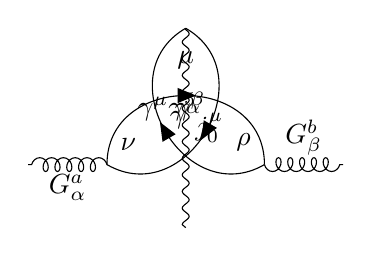
\begin{tikzpicture}
  \begin{feynman}
    % Define vertices
    \vertex (a) at (0, 0);
    \vertex (b) at (2, 0);
    \vertex (c) at (1, 1.732); % 60-degree triangle height
    \vertex (d) at (-1, 0);    % Left gluon
    \vertex (e) at (3, 0);     % Right gluon
    \vertex (f) at (1, -0.8);  % Axial current

    % Draw propagators with labels
    \diagram*{
      (a) -- [fermion, half left, edge label'=$\gamma^\alpha$] (b)
        -- [fermion, half left, edge label'=$\gamma^\beta$] (c)
        -- [fermion, half left, edge label'=$\gamma^\mu \gamma^5$] (a),
      (a) -- [gluon, edge label=$G^a_\alpha$] (d),
      (b) -- [gluon, edge label=$G^b_\beta$] (e),
      (c) -- [boson, edge label=$j_0^\mu$] (f)
    };

    % Annotate vertices (optional)
    \node at (a) [above right=2pt] {\(\nu\)};
    \node at (b) [above left=2pt] {\(\rho\)};
    \node at (c) [below=5pt] {\(\mu\)};
  \end{feynman}
\end{tikzpicture}
\end{document}